\documentclass{article}
% packages
\usepackage {lmodern}
\usepackage [T1]{fontenc}
\usepackage {amsmath}
\usepackage {amssymb}
\usepackage {amsfonts}
\usepackage {graphicx}
\usepackage {fullpage}
\usepackage {gensymb}
\usepackage {caption}
\usepackage {subcaption}
\usepackage {array}
%\usepackage{nopageno}
\usepackage {cite}
\usepackage {setspace}
\usepackage [version=4]{mhchem}
\usepackage {pdfpages}
\usepackage [ampersand]{easylist}
\usepackage {fancyvrb}
\usepackage {listings}
\usepackage {color}

\definecolor{dkgreen}{rgb}{0,0.6,0}
\definecolor{gray}{rgb}{0.5,0.5,0.5}
\definecolor{mauve}{rgb}{0.58,0,0.82}

\lstset{frame=tb,
	language=C,
	aboveskip=3mm,
	belowskip=3mm,
	showstringspaces=false,
	columns=flexible,
	basicstyle={\small\ttfamily},
	numbers=none,
	numberstyle=\tiny\color{gray},
	keywordstyle=\color{blue},
	commentstyle=\color{dkgreen},
	stringstyle=\color{mauve},
	breaklines=true,
	breakatwhitespace=true,
	tabsize=3
}


\usepackage{titling}
\newcommand{\subtitle}[1]{%
    \posttitle{%
        \par\end{center}
        \begin{center}\LARGE#1\end{center}
        \vskip0.5em}%
}

\graphicspath {{images/}}

\begin{document}
\title{An Investigation on the Efficiency of Sequence Alignment Tools}
\subtitle{Final Report}
\author {Justin Chao - juchao \\
		Chase Meyer - cmeyer3 \\
		Bria Lacour - lacour}
\maketitle
\vspace{4cm}
\section*{Abstact} 
A Sequence Alignment program that utilizes a global alignment algorithm to
optimize protein sequence alignments was developed and its computational
efficiency was compared to other open source and industry standard programs.
 
Given mismatch, gap penalty, and match scoring parameters, a similarity matrix is
dynamically generated using the Needleman-Wunsch algorithm between two
user-provided sequences.  
The two sequences may then be scored according to user-provided scoring
parameters.

Execution of the BSD time command reveals a real time of 0.024 seconds for our
dynamically programmed code, as compared to a time of 0.026 seconds for another
open source sequence alignment program.

\newpage

\section*{Introduction}
Sequence alignment (SA) tools are used by computational biologists to track evolutionary
relationships, mutations, and predict structure vs. function relationships among living
systems. These tools can be used to assist in the identification of patterns in protein
families, prove homology, and assess conservation in genetic characteristics across species.
Figure \ref{fig:ma} illustrates a multiple sequence alignment analysis of
different protein sequences.

\begin{center}
    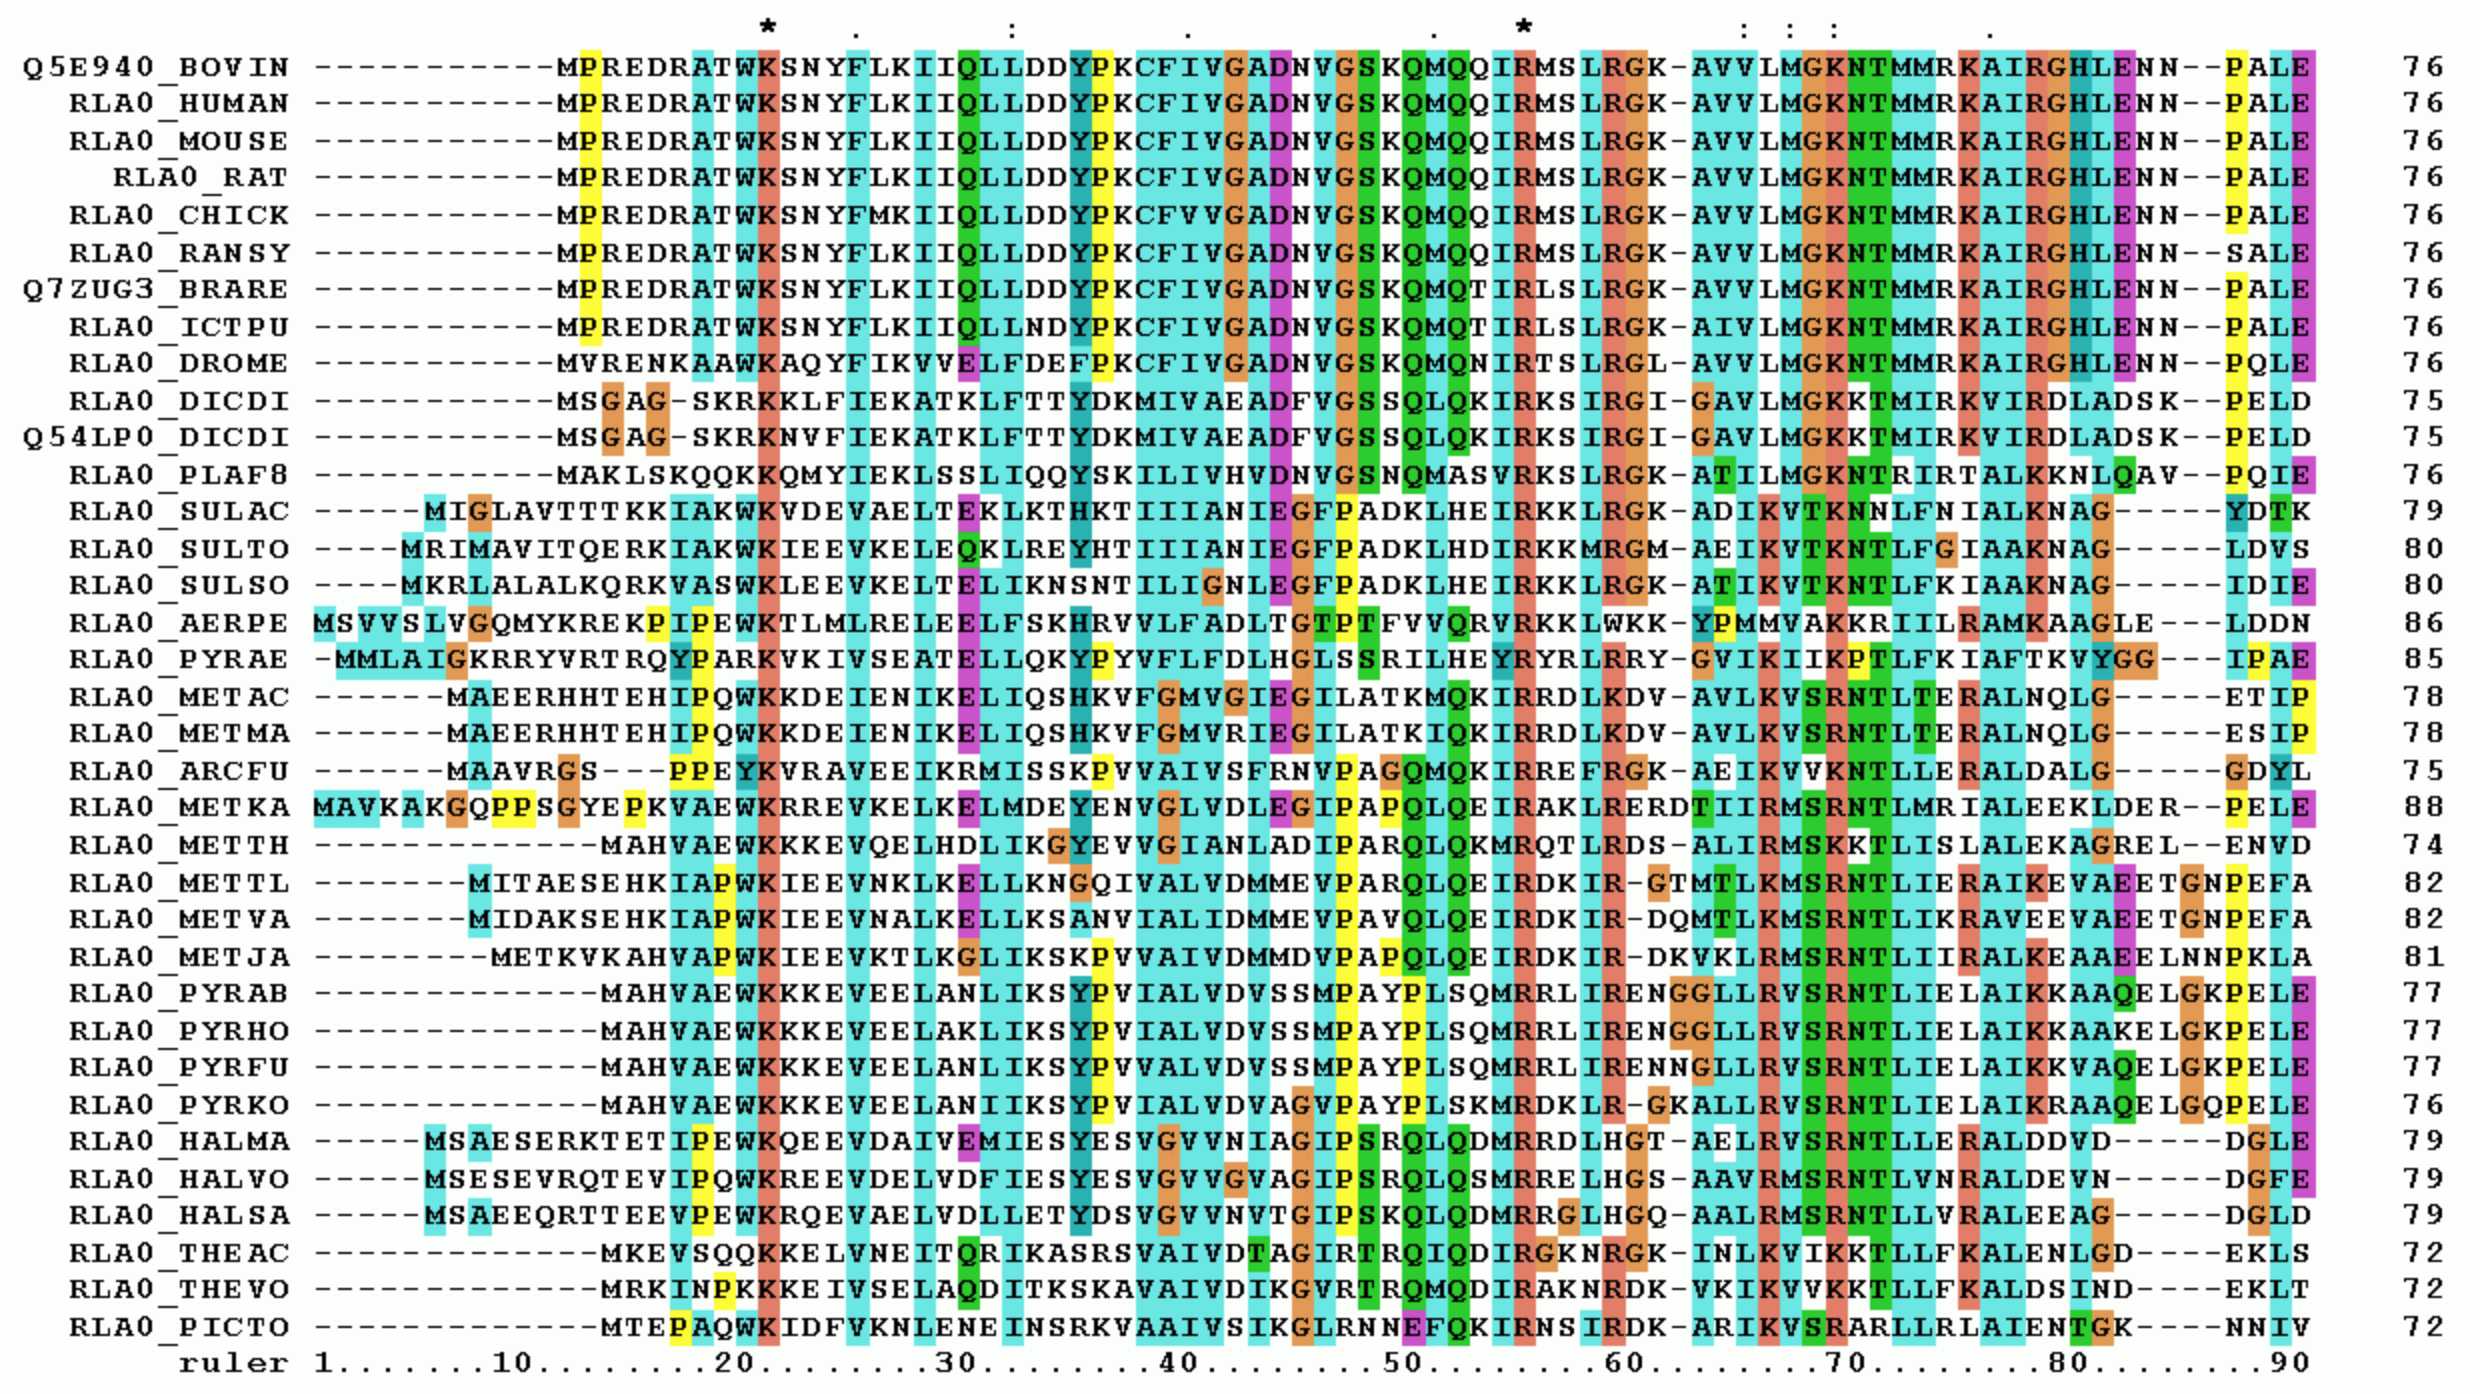
\includegraphics[scale=0.35]{multiple_alignment}
    \captionof{figure}{Representation of a protein multiple sequence alignment
    produced with ClustalW. The sequences are instances of the acidic ribosomal
    protein P0 homolog (L10E) encoded by the Rplp0 gene from multiple organisms.
    Only the first 90 positions of the alignment are displayed. The colors represent the
    amino acid conservation according to the properties and distribution of
    amino acid frequencies in each column. Note the two completely conserved
    residues arginine (R) and lysine (K) marked with an asterisk at the top of
    the alignment. \cite{multiple_alignment}}
    \label{fig:ma}
\end{center}

Sequences of interest are usually protein, DNA, or RNA chains.  For different
sequence types, different analytical methods must be employed for comparison.
Therefore, SA tools are often found in a variety of forms, tailored to address
specific biological problems. \cite{rosenburg}

Depending on the desired level of accuracy and computational efficiency, there
are many different types of alignment methods. 
Global alignments attempt to align and match every residue or nucleotide in each
sequence, making them better suited for more similar and equal-sized sequences.
Local alignments are better suited for locating smaller subsequences that match
between two sequences. For proteins, this could indicate a shared protein family
and similar domains of interest and function. 
However, analyzing local alignments requires additional levels of complexity and
constraint parameters, which can drastically increase computational costs. \cite{nguyen} 

Due to the complexity and length of most sequences of interest, the
computational efficiency of SA tools is of particular importance.  This project
will analyze the Needleman-Wunsch algorithm for assessing the global alignment
of two sequences, and compare the efficiency of the algorithm with other open
source, global alignment SA tools.


\subsection*{Needleman-Wunsch Algorithm}
The Needleman-Wunsch algorithm is a global alignment method used in many
sequence alignment tools. The algorithm compares two sequences by dynamically
generating a similarity matrix with scoring values calculated based
user-provided parameters.

Equation 1 defines the Needleman-Wunsch algorithm.

\begin{align*}
    M(0, j) = j \times p  \hspace{1cm}&\text{for first row, where p is the gap
    penalty} \\
    M(i, 0) = i \times p  \hspace{1cm}&\text{for first column}
\end{align*}

\begin{equation}
    M(0, j) = max \begin{cases}
        M(i-1, j) + p & \text{top} \\
        M(i, j-1) + p & \text{left} \\
        M(i-1, j-1) + s(a_j , b_i) & \text{diagonal}
  \end{cases}
\end{equation}

Where $s(a_j , b_i)$ = match/mismatch score for sites j and i in sequences a and
b. \cite{columbia}

Figure \ref{fig:nw} provides a graphical illustration of how the Needleman-Wunsch
algorithm populates a similarity matrix of scoring values.

\begin{center}
    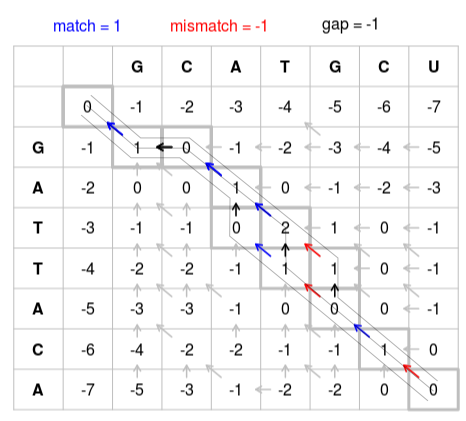
\includegraphics[scale=0.7]{nw.png}
    \captionof{figure}{Needleman-Wunsch pairwise sequence alignment. \cite{nw}}
    \label{fig:nw}
\end{center}

The gray arrows represent the filling of each position in the matrix by the
match. mismatch, or gap scores. This algorithm starts at zero in one corner of
the matrix (second row, second column). In order to determine the score of a
particular position in the matrix, the corresponding residue in its column
(sequence 1) and its row (sequence 2) are compared. Each of the positions beside
the position is scored and the highest existing score calculated goes in the
current position. For the second row, we add 0, -1, -2, -3, -4, -5, -6, -7 due
to the lack of top and top-left cells. Then, in order to find the best
alignment, we backtrack to the origin by following the arrows. The alignment is
constructed by allowing the diagonal arrows to represent match or mismatches,
horizontal arrows to represent gaps after the letter, and vertical arrows to
represent a gap after the letter in the top sequence. \cite{nw}

\section*{Methodology and Results} 

All code was run on the TACC Lonestar5 system, with TP53 protein sequences for
Mouse and Humans as comparison sequences.  
The GNU GDB debugger was used in the debugging and analysis of the code, and 
the Intel ICC compiler was used to compile the code.

Table \ref{tab:data} compares execution time under the BSD time command of our
code with other SA programs.

\begin{center}
    \captionof{table}{Comparison of Execution Times to Other SA Tools}
    \begin{tabular}{c|c|c|c|c|c}
        & Open Source Code - NW & Ours - NW & MAFFT & MUSCLE & Clustal Omega \\
        \hline
        Real Time (s) & 0.026 & 0.024 & 0.004 & 0.014 & 0.005 \\
        User Time (s) & 0.016 & 0.016 & 0.000 & 0.004 & 0.000 \\
        System Time (s) & 0.006 & 0.004 & 0.000 & 0.004 & 0.000 \\
    \end{tabular}
    \label{tab:data}
\end{center}

Dynamic generation of the similarity matrix allows for a slight increase in
computational efficiency for our code, as compared with other open source codes.

Figures \ref{fig:flat_profile} and \ref{fig:call_graph} show the flat profile
and call graph as generated from GNU gprof for our code.

\begin{center}
    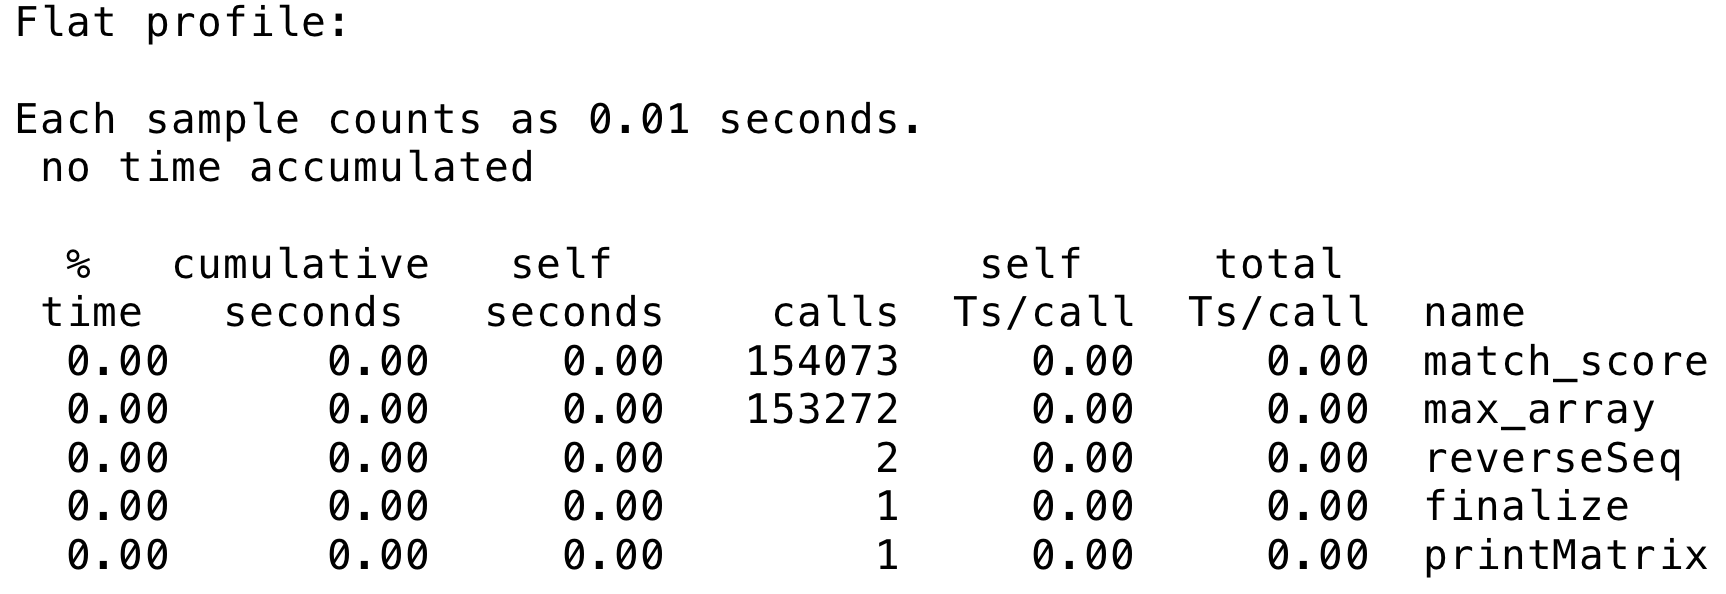
\includegraphics[scale=0.4]{flat_profile.png}
    \captionof{figure}{Flat profile of needleman\_wunsch code.}
    \label{fig:flat_profile}

    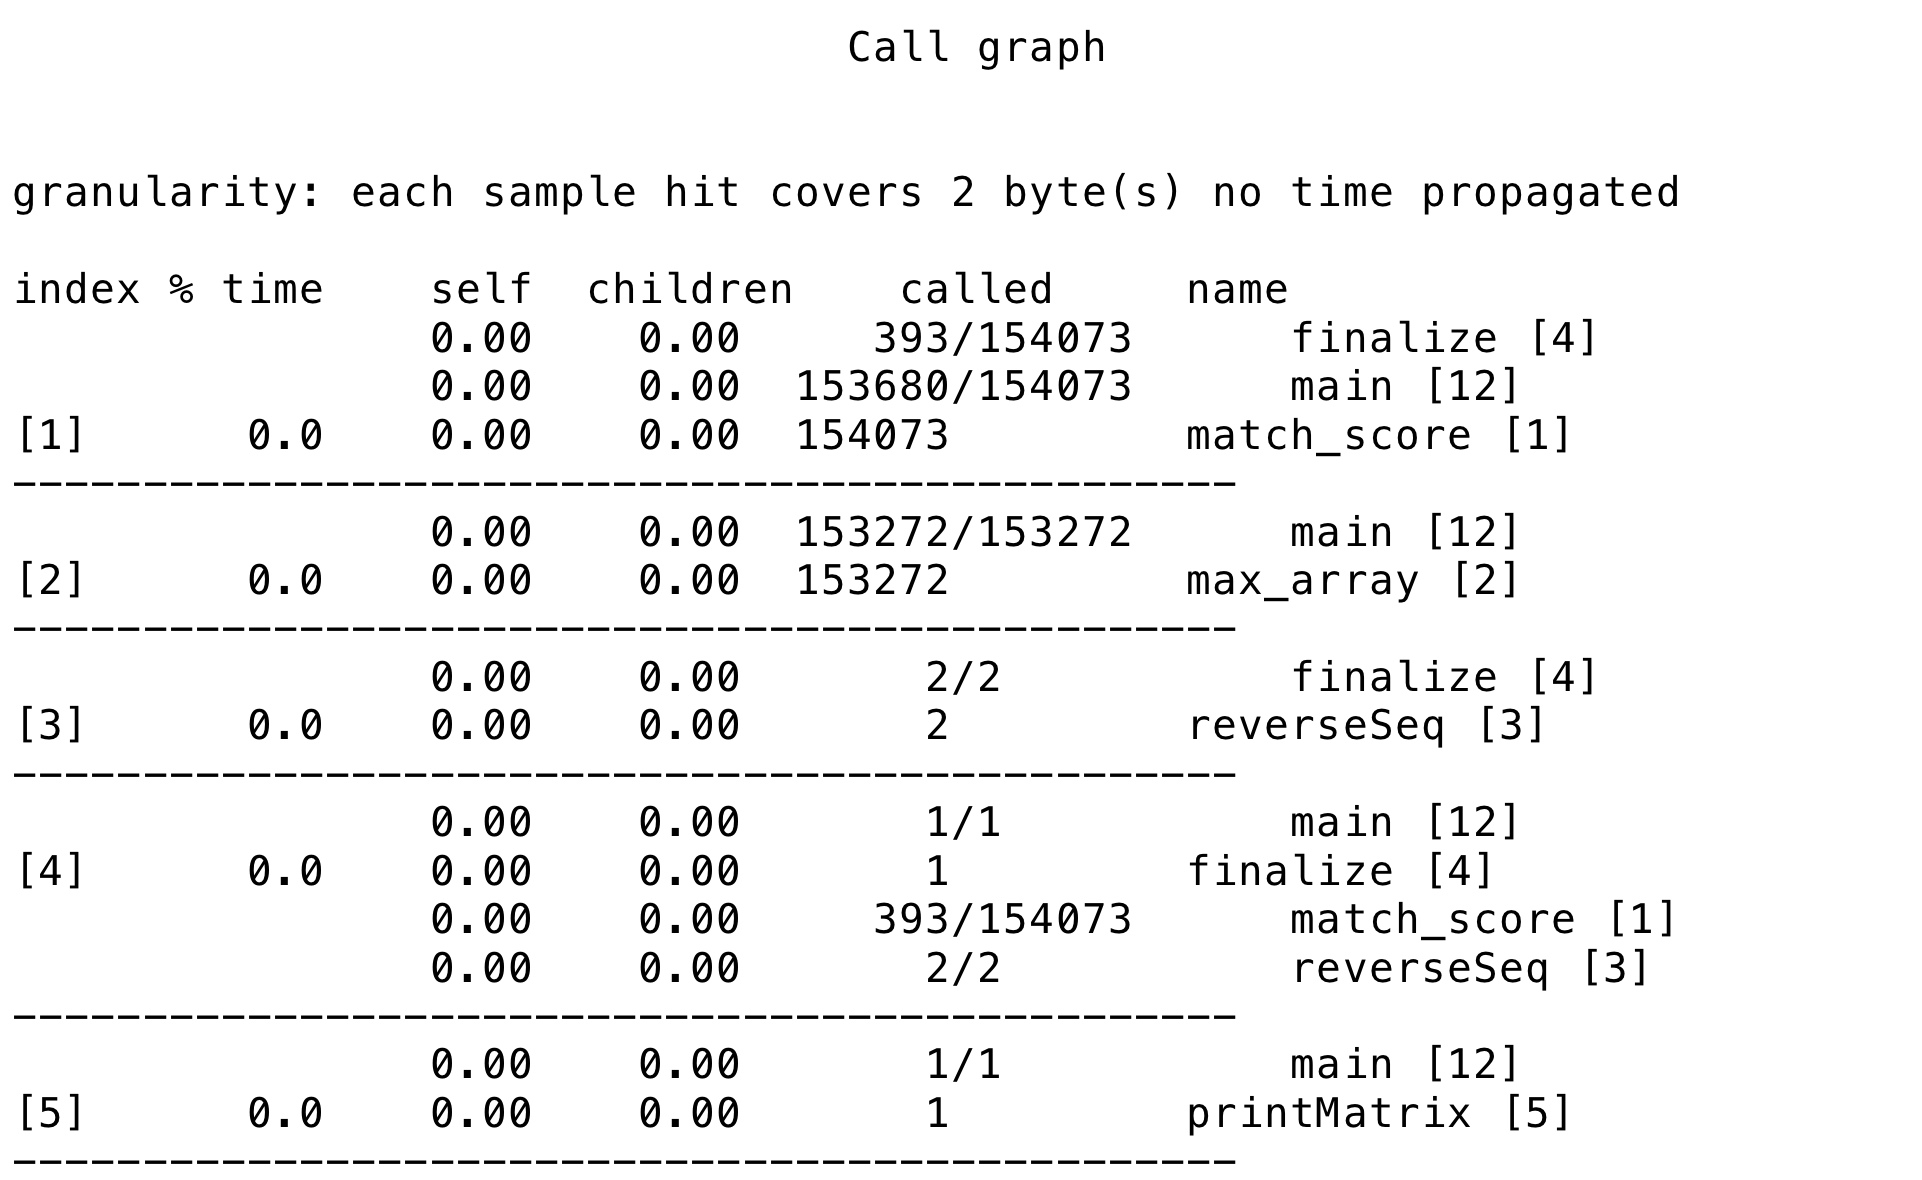
\includegraphics[scale=0.4]{call_graph.png}
    \captionof{figure}{Call graph of needleman\_wunsch code.}
    \label{fig:call_graph}
\end{center}

Our code was continuously profiled and restructured to allow for better 
efficiency between function calls and code execution, thereby decreasing
computational costs.

Figures \ref{fig:human_rat} and \ref{fig:human_human} show output examples from our code comparing
TP53 protein subsequences from mouse and human specimens.

\begin{center}
    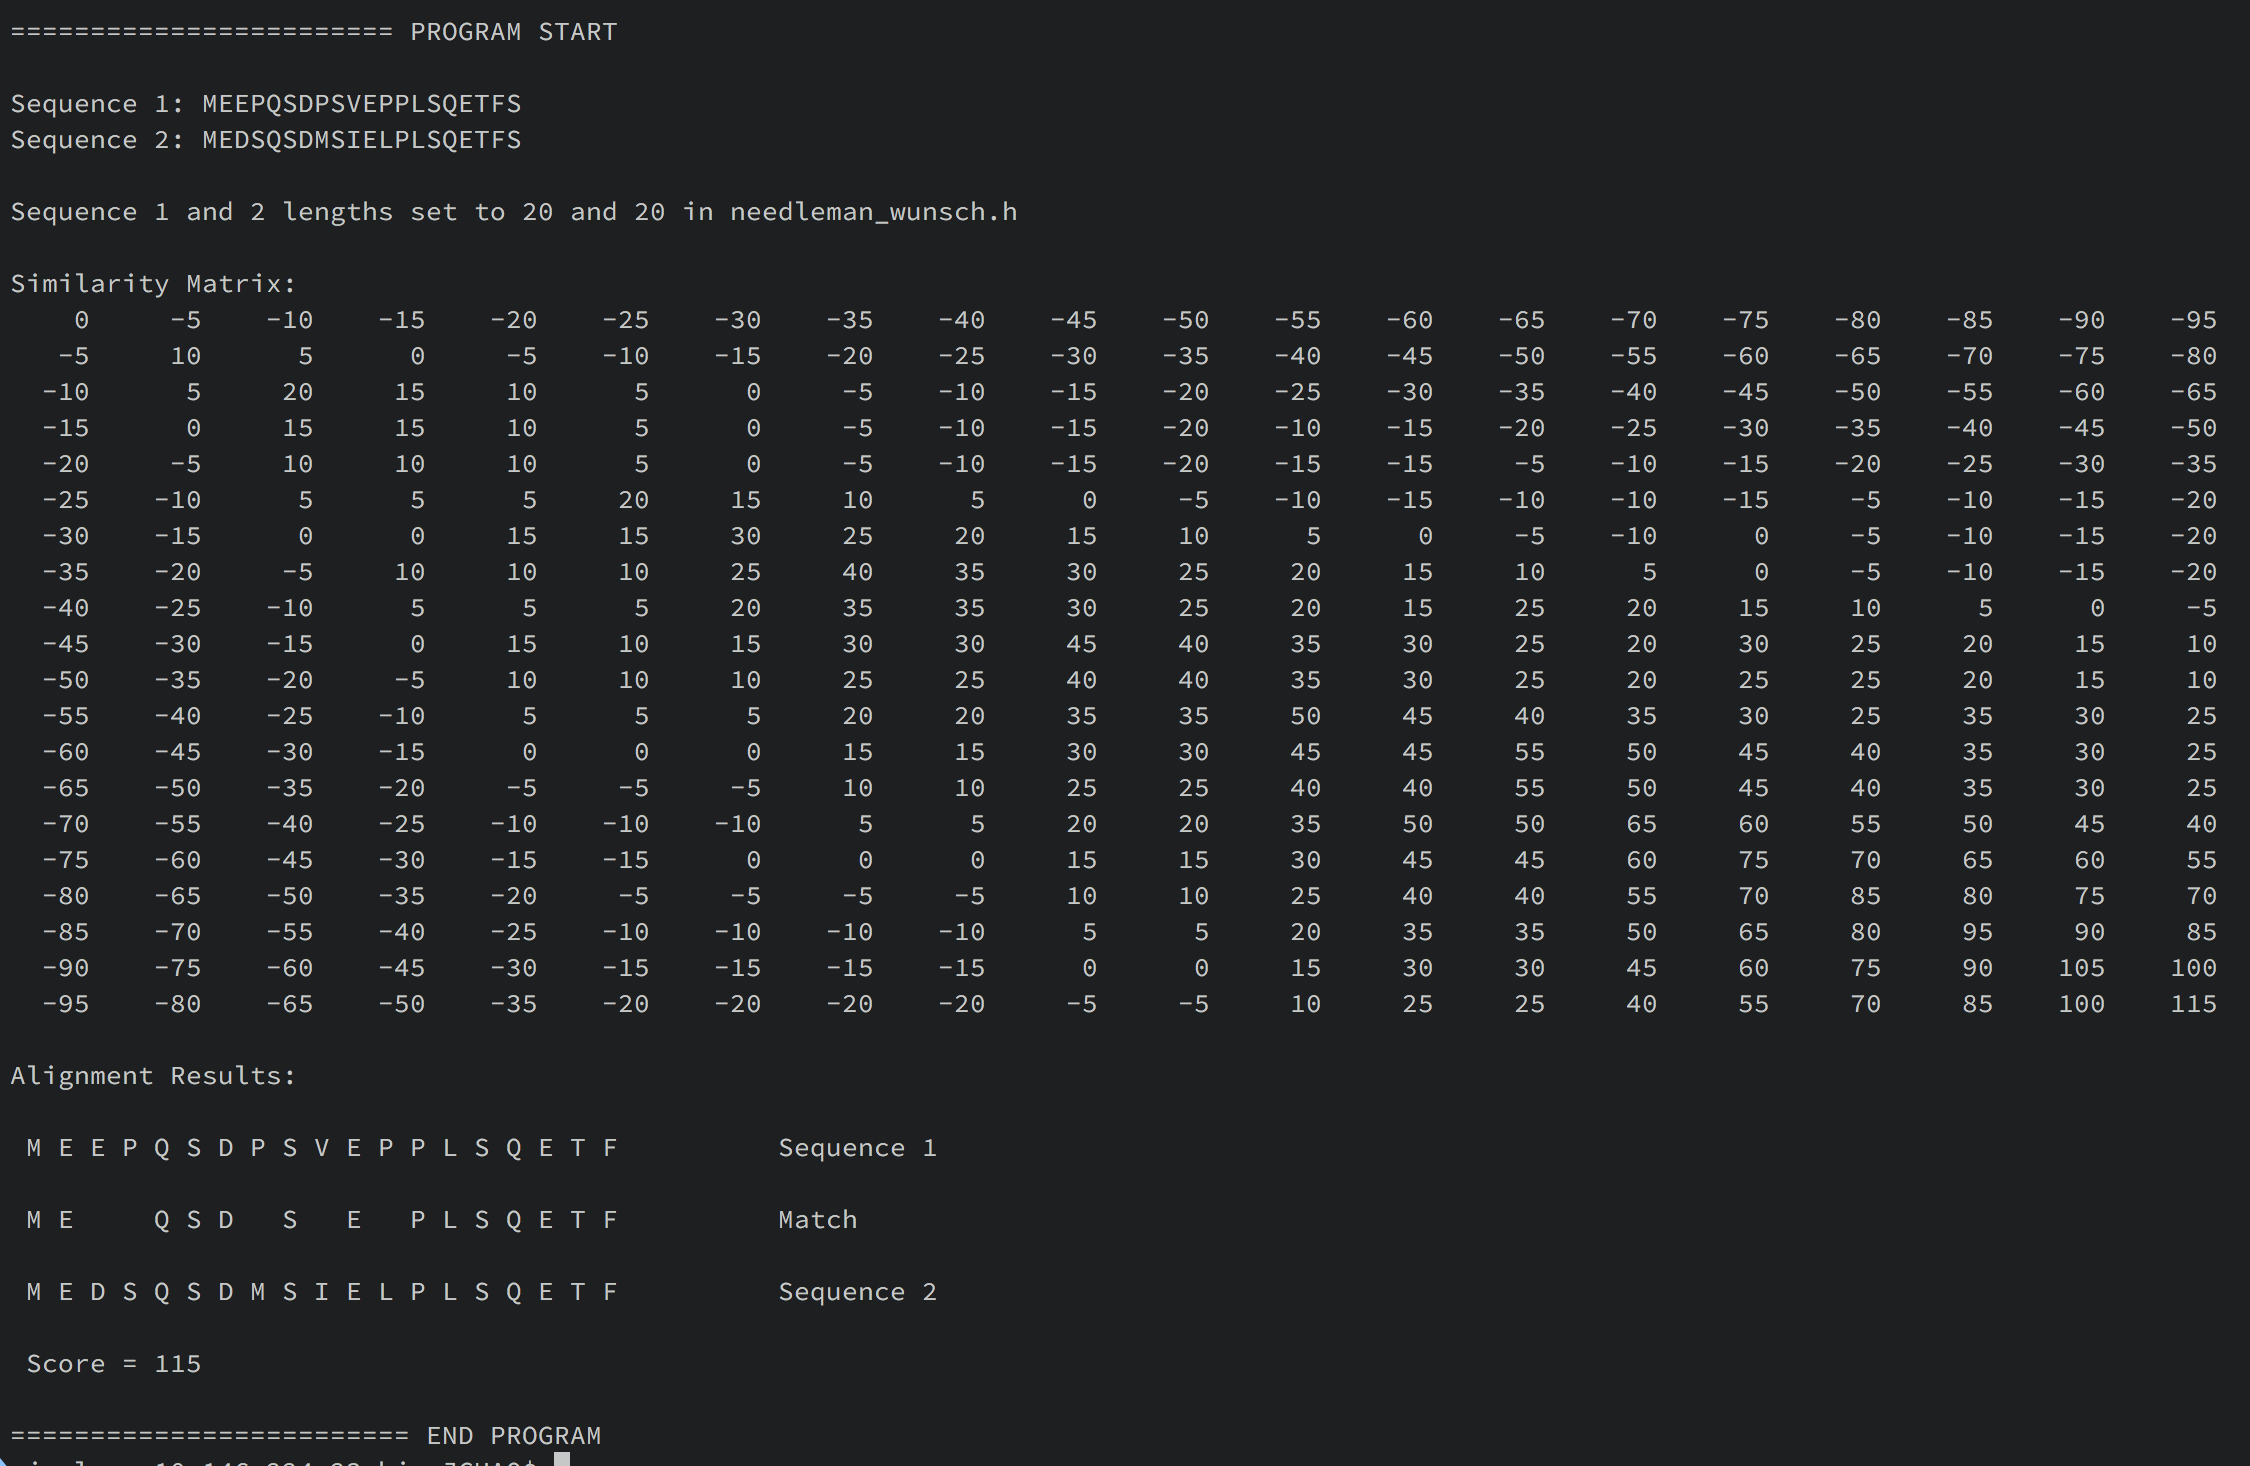
\includegraphics[scale=0.35]{human_rat}
    \captionof{figure}{Sample output comparing a subsequence of TP53 protein in
    human vs. rat.}
    \label{fig:human_rat}

    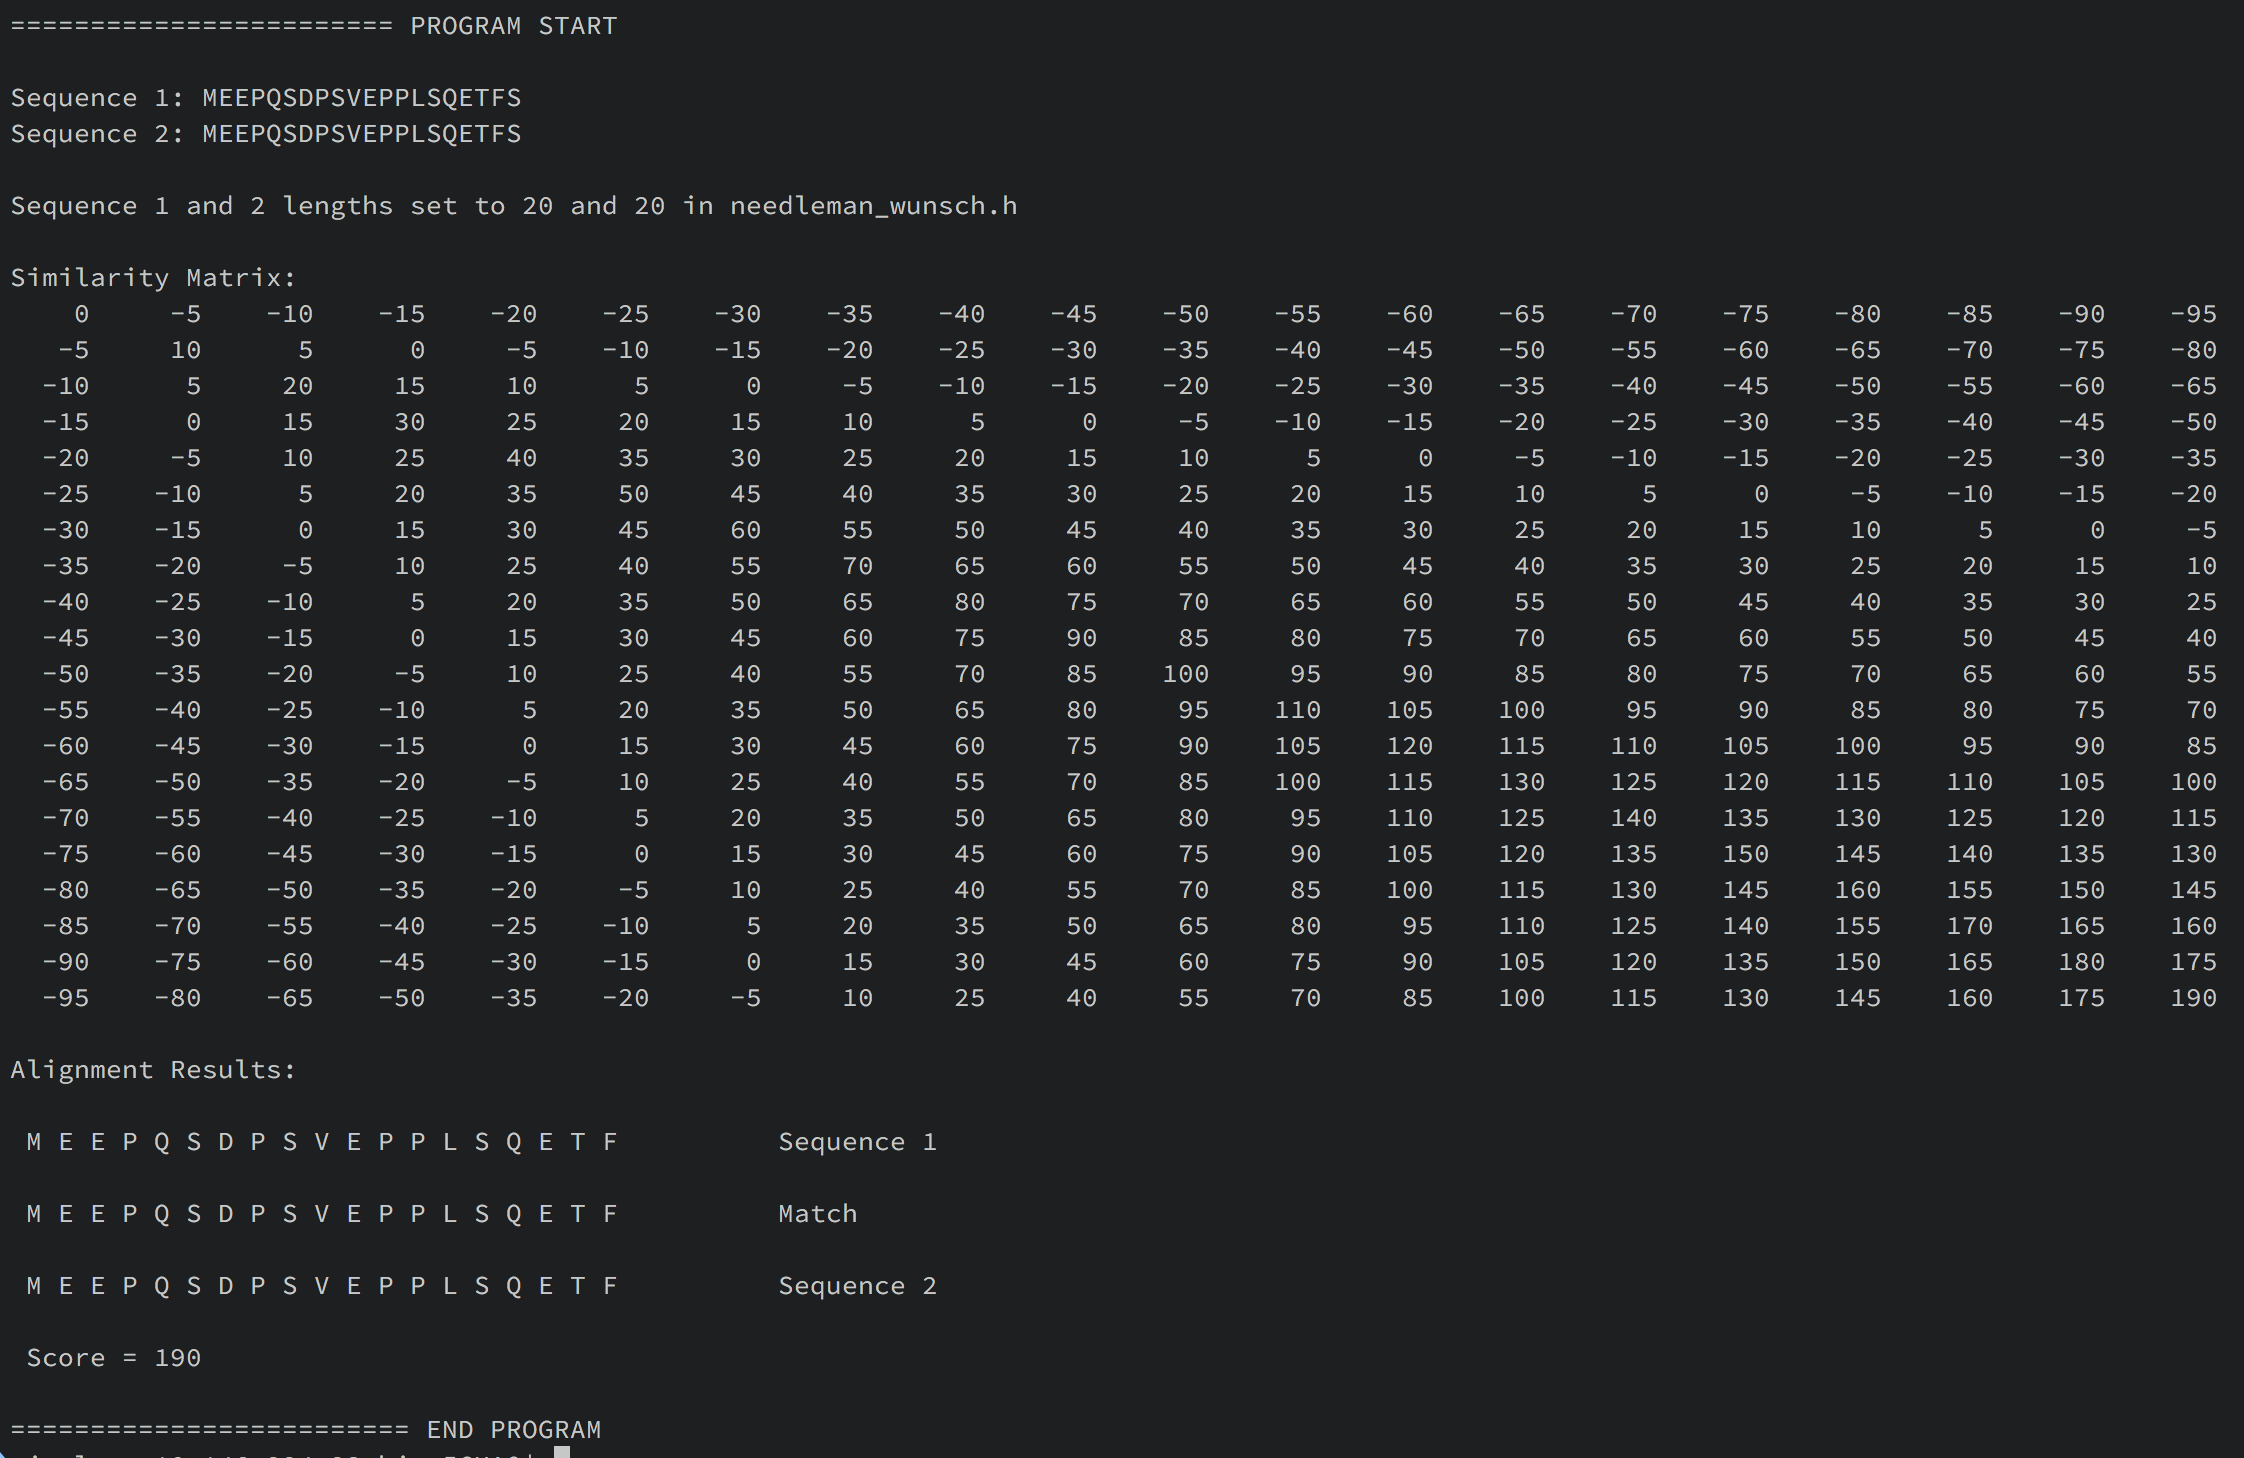
\includegraphics[scale=0.35]{human_human}
    \captionof{figure}{Sample output comparing a subsequence of TP53 protein in
    human vs. human.}
    \label{fig:human_human}
\end{center}


\section*{Discussion}
We initially proposed to compare our sequence alignment tool with other
industry standard SA tools used by bioinformaticians. 
However, further investigation into how industry standard tools operate reveal the
use of multiple alignment algorithms, as well as machine learning software and
protein family prediciton tools for further optimization.

Since our alignment tool only utilizes a global alignment algorithm, an open
source code also written in C was found for comparison purposes.
A comparison of execution and run times between our code and the open source
code revealed increases in computational efficiency and speed.

\section*{Conclusion}
A sequence alignment program that utilizes the Needleman-Wunsch algorithm to
globally align protein sequences was developed, and its
computational efficiency was compared to other industry standard programs.
 
Tools such as GNU GDB and gprof were used to debug and profile our code.
Execution of the BSD time command reveals increases in computational efficiency
as compared to other open source programs.

Future studies may include analysis of optimization differences accross
different compilers.

\newpage
\section*{Appendix}
The following contains source code taken from our program.
\subsubsection*{main.c}
\begin{lstlisting}
// main.c file for needleman_wunsch alignment program
#include "needleman_wunsch.h"
#include <stdio.h>
#include <stdlib.h>

// define scoring parameters
#define gap_penalty -5

#define A(i,j) score[(i) + (j)*n]

// variable declarations
int i, j, k, l, count = 0;
int score_current = 0, score_diagonal = 0, score_up = 0, score_left = 0;
int sizeAlign1 = 0;
int sizeAlign2 = 0;

// main.c takes two sequences as command line arguments
int main(int argc, char *argv[]) {

    // allocating plenty of memory to store each of the sequences 
    char *align1 = malloc(500*sizeof(char));  
    char *align2 = malloc(500*sizeof(char));

    if (argc != 3) {
        printf ("\nUsage: \n./Needleman_Wunsch <sequence1> <sequence2>\n\n");
        return 0;
    }

    printf("\n======================== PROGRAM START \n\n");

    int values[3];
    char seq1[m], seq2[n];

    // print sequences and user-defined lengths
    for (i=1; i<argc; i++)
        printf("Sequence %d: %s\n", i, argv[i]);  
    printf("\nSequence 1 and 2 lengths set to %d and %d in needleman_wunsch.h\n", m, n);

    // assign command line arguments to array of chars for each sequence
    for (i=0; i<=m; i++)
        seq1[i] = argv[1][i];
    for (i=0; i<=n; i++)
        seq2[i] = argv[2][i];

    // allocate memory for scoring matrix
    int *score = malloc ((m + 1)*(n + 1)*sizeof(int));

    // initially set all values to 0
    for (i=0; i< m; i++) 
        for (j=0; j< n; j++)
            A(i,j) = 0;
   
    // fill in first row
    for (k=0; k<n; k++) 
        A(0,k) = gap_penalty * k;

    // fill in first column
    for (l=0; l<m; l++)
        A(l,0) = gap_penalty * l;
    
    // fill in other values
    for (i=1; i<m; i++) {
        for (j=1; j<n; j++) {
            values[0] = A(i-1, j) + gap_penalty;
            values[1] = A(i, j-1) + gap_penalty;
            values[2] = A(i-1, j-1) + match_score (seq1[i-1], seq2[j-1]);
            A(i,j) = max_array(values, 3);
        }
    }

    // print Similarity Matrix
    printf ("\nSimilarity Matrix: ");
    printMatrix(score);

    // begin traceback
    i = m - 1;
    j = n - 1;

    while (i>0 && j>0) {
        score_current = A(i,j);
        score_diagonal = A((i-1),(j-1));
        score_up = A((i),(j-1));
        score_left = A((i-1),(j));

        if (score_current == score_diagonal + match_score(seq1[i-1], seq2[j-1])) {
            align1[count] = seq1[i-1];
            align2[count] = seq2[i-1];
            i --;
            j --;
            sizeAlign1 ++;
            sizeAlign2 ++;
            count ++;
        }
        else if (score_current == score_left + gap_penalty) {
            align1[count] = seq1[i-1];
            align2[count] = '-';
            i --;
            sizeAlign1 ++;
            sizeAlign2 ++; 
            count ++;
        }
        else if (score_current == score_up + gap_penalty) {
            align1[count] = '-';
            align2[count] = seq2[j-1];
            j --;
            sizeAlign1 ++;
            sizeAlign2 ++;
            count ++;
        }
    }
    
    // finish tracing up to top left cell
    while (i > 0) {
        align1[count] = seq1[i-1];
        align2[count] = '-';
        i --;
        sizeAlign1 ++;
        sizeAlign2 ++;
        count ++;
    }
    while (j > 0) {
        align1[count] = '-';
        align2[count] = seq2[j-1];
        j --;
        sizeAlign1 ++;
        sizeAlign2 ++;
        count ++;
    } 

    finalize (align1, align2, sizeAlign1, sizeAlign2);

    printf("\n========================= END PROGRAM \n");
    return 0;
}
\end{lstlisting}

\newpage
\subsubsection*{needleman\_wunsch.h}
\begin{lstlisting}
// needleman_wunsch.h header file for needleman_wunsch alignment program

#ifndef needleman_wunch_h   // Include guard
#define needleman_wunch_h

#define m 20    // m = length of Sequence 1
#define n 20    // n = length of Sequence 2

int match_score(char a, char b);
int max_array (int a[], int num_elements);
void printMatrix (int matrix[m*n]);
void reverseSeq (char arr[], int start, int end);
void finalize (char align1[], char align2[], int sizeAlign1, int sizeAlign2);

#endif
\end{lstlisting}

\newpage
\subsubsection*{needleman\_wunsch.c}
\begin{lstlisting}
// needleman_wunsch.c file for needleman_wunsch alignment program
#include "needleman_wunsch.h"
#include <stdio.h>
#include <stdlib.h>

// define scoring parameters
#define gap_penalty -5
#define matchScore  10
#define mismatch -5

int match_score(char a, char b) {
    int m_score, i, a_num, b_num;
    if (a == b)
      return matchScore;
    else if (a == '-' || b == '-') 
      return gap_penalty;
    else // there is a mismatch
      return mismatch;
}

int max_array (int  a[], int num_elements) {
    int i, max=-5000;
    for (i=0; i<num_elements; i++)
        if (a[i]>max) max = a[i];
    return max;
}

void printMatrix (int matrix[m*n]) {
    int i, j; 
    printf ("\n"); 
    for (i=0; i<m; i++){
        for (j=0; j<n; j++)
            printf ("%5.1d  ", matrix[i+j*m]);
        printf ("\n");
   }
}

void reverseSeq(char arr[], int start, int end) {
    int temp;
    while (start < end) {
        temp = arr[start];   
        arr[start] = arr[end];
        arr[end] = temp;
        start ++;
        end --;
    }   
}    

void finalize (char align1[], char align2[], int sizeAlign1, int sizeAlign2) {
    int i;
    // reverse sequences
    reverseSeq (align1, 0, sizeAlign1);
    reverseSeq (align2, 0, sizeAlign2);
    
    char *symbol = malloc(500*sizeof(char));

    int scoreNum = 0, count = 1;

    for (i=1; i<=sizeAlign1; i++){
        // if two AAs are the same, output the letter
        if (align1[i] == align2[i]) {
            symbol[count] = align1[i];
            scoreNum = scoreNum + match_score(align1[i], align2[i]);
            count ++;
        }
        // if they are not identical and none of them is gap
        else if (align1[i] != align2[i] && align1[i] != '-' && align2[i] != '-') {
            scoreNum = scoreNum + match_score(align1[i], align2[i]);
            symbol[count] = ' ';
            count ++;
        }
        // if one of them is a gap, output a space
        else if (align1[i] == '-' || align2[i] == '-') {
            symbol[count] = ' ';
            scoreNum = scoreNum + gap_penalty;
            count ++;
        }
    }

    printf ("\nAlignment Results:\n\n");
    for (i=0; i<=sizeAlign1; i++) printf ("%c ", align1[i]);

    printf ("\t\tSequence 1\n\n");
    for (i=0; i<=count; i++) printf ("%c ", symbol[i]);

    printf ("\tMatch\n\n");
    for (i=0; i<=sizeAlign2; i++) printf ("%c ", align2[i]);

    printf ("\t\tSequence 2\n");

    printf ("\n Score = %d\n", scoreNum);
}
\end{lstlisting}





\newpage
\bibliographystyle{unsrt}
\bibliography{final_report.bib}

\end{document}
